%-------------------------------------------------------------------------------
\section{Reusing Already Built Packages}
%-------------------------------------------------------------------------------
\label{sec:reuse}

While \spack{} is primarily a package manager installing software \emph{from sources},
the ability to reuse already built software and mix it seamlessly with source builds has
been a critical request from the community for several years.

\begin{figure}[t]
  \centering
  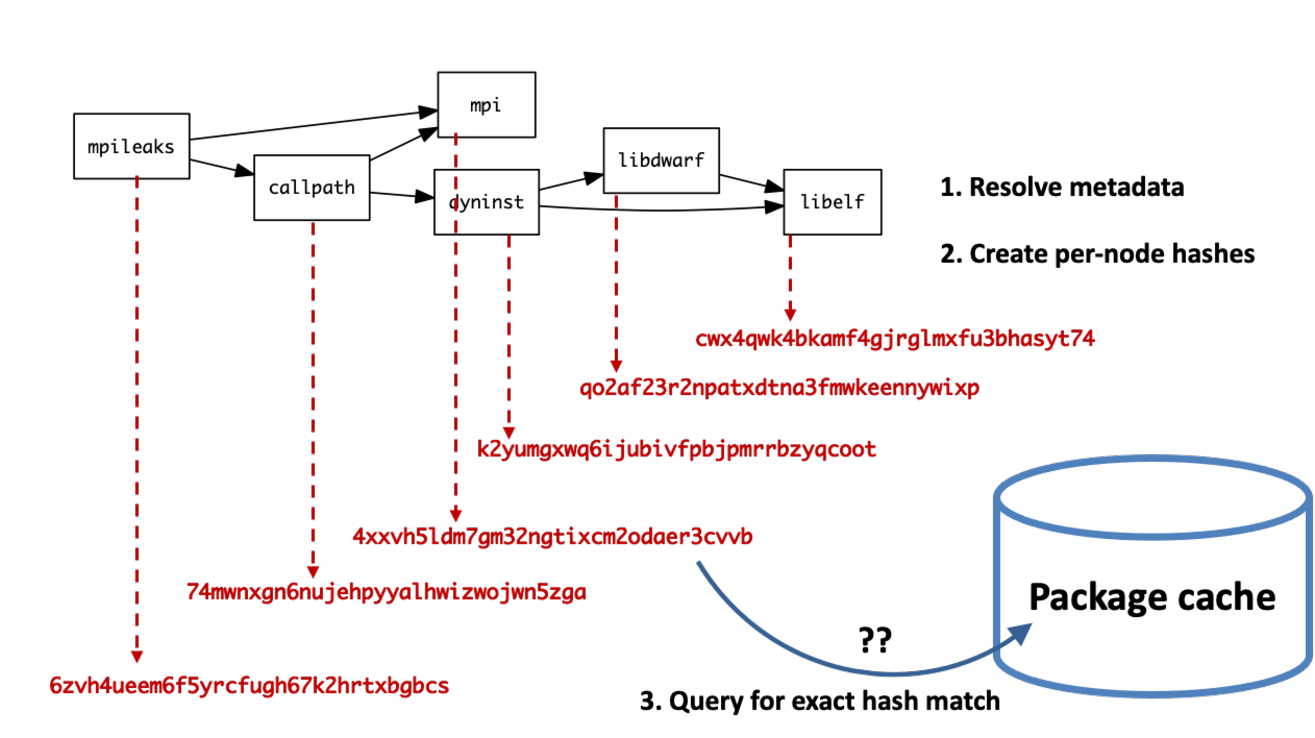
\includegraphics[width=\columnwidth]{figures/hash-cache.pdf}
  \caption{
    Hash-based reuse in the original \spack concretizer.
    \label{fig:hash_reuse}
  }
\end{figure}

Functional packaging systems, including \spack{} with the old concretizer, reuse builds
via metadata hashes. This mechanism relies on the fact that, when an installation graph
is concretized, each node in the DAG is given a unique hash, as shown in
Figure~\ref{fig:hash_reuse}.
%A user can then query for an exact hash match to reuse
%something that is either already installed or available as a binary package.
Unless the user was explicit, \spack{} only reused packages if their hashes matched
exactly. Small configuration changes could easily result in little or no reuse.

%The issue with this way of proceeding is that users are \emph{effectively
%overconstraining} their request since specifying the hash is equivalent to specifying
%\emph{all the metadata} of the associated spec. This exposes users to need frequent
%changes in their configuration, since hashes are very sensitive to small changes, and
%prevents them from finding other satisfying specs that might be available.
% FIXME: expand on Nix, Guix, Conan etc. ?

%\subsection{Optimizing for Software Reuse}

A more effective way to approach software reuse can be achieved by leveraging the
``Generalized Condition Handling'' logic described in
Section~\ref{subsec:generalizedcond}. First, all the metadata from installed packages
can be encoded into facts:
\begin{minted}[fontsize=\footnotesize, bgcolor=bg]{prolog}
installed_hash("zlib","7fatd...").
imposed_constraint("7fatd...","node","zlib").
imposed_constraint("7fatd...","version","zlib","1.2.11").
imposed_constraint("7fatd...","node_platform","zlib","linux").
imposed_constraint("7fatd...","node_os","zlib","ubuntu20.04").
imposed_constraint("7fatd...","node_target","zlib","icelake").
...
\end{minted}
The encoding is based on \texttt{imposed\_constraint}, but the constraint ID is the
hash associated with the installed package. To minimize the number of builds from
source, the solver is allowed to choose a hash to resolve any package:
\begin{minted}[fontsize=\small, bgcolor=bg]{prolog}
{hash(P, Hash) : installed_hash(P, Hash)} 1 :- node(P).
\end{minted}
Impose all constraints associated with chosen hashes:
\begin{minted}[fontsize=\small, bgcolor=bg]{prolog}
impose(Hash) :- hash(P, Hash).
\end{minted}
And number of builds (packages \emph{without} a hash) is minimized:
\begin{minted}[fontsize=\small, bgcolor=bg]{prolog}
build(P) :- not hash(P, _), node(P).
#minimize { 1@100,P : build(P) }.
\end{minted}

This is a remarkably simple encoding for a complex constraint problem that cannot be
solved with the prior greedy concretizer. However, the devil is in the details.
Minimizing builds can have two effects---it can cause the concretizer to prefer an
existing installation over building a new version of a package, but if set as the
highest optimization priority, it also causes the concretizer to configure newly built
packages in any way that {\it minimizes dependencies}. Generally, though, users expect
new builds to use regular defaults---i.e., most recent version, preferred variants, etc.
As an illustrative example, building \texttt{cmake} with these objectives will build
{\it without} networking capabilities, because it omits \texttt{openssl} and its
dependencies from the graph!

%The
%trickiest point is how to choose at which priority the minimization of builds should be
%put in our multi-objective optimization criteria. The difficulty we face here stems from
%the different nature that an already built configuration has with respect to one that we
%still have to build. In the former case we can't change any aspect of the underlying
%graph, e.g. we can't choose a different version or a different set of variants to
%improve some optimization score, since the installed configuration is immutable. In the
%latter case instead, since we still have to build the software, we would like to choose
%the most recent version, use the preferred variants etc.

%% Reasoning on this issue it becomes evident that having a single optimization criteria
%% that accounts for both installed and non-installed software would always lead to
%% unsatisfying behavior. For instance, if we optimized for minimizing builds at the
%% highest priority and have no installed software to reuse, the solver would choose
%% minimal DAGs even though that means using old versions or non-default values for
%% variants. If a user asked to build e.g. \texttt{cmake} it would probably be unexpected
%% to build one version without networking capabilities just because that permits to trim
%% \texttt{openssl} and its dependencies from the graph!

Our solution is to split the optimization criteria into two identical ``buckets'', one
for installed software and one for software that is yet to be built, and optimize for
them at different priorities:
\begin{enumerate}
\item Minimize all objectives for software to be built
\item Then, minimize the number of builds
\item Minimize the objectives for already built software
\end{enumerate}
Minimizing the number of builds at a priority that is always higher than any other
criteria for installed software, but always lower than any criteria for software to be
built allows \spack{} to pick the best version available from what is installed without
adversely affecting the choice of defaults for built packages. This is actually simple
to encode in ASP:

\begin{minted}[fontsize=\footnotesize, bgcolor=bg]{prolog}
build_priority(P, 200) :- build(P), node(P).
build_priority(P, 0)   :- not build(P), node(P).
% ....
#minimize{
    W@5+Priority,P
    : version_weight(P, W), build_priority(P, Priority)
}.
\end{minted}

Here, {\tt Priority} will be 200 for built packages and 0 for preinstalled packages, and
we can use this to control the priority of the minimization objective. This {\tt
  \#minimize} sums into {\it two} buckets in a global per-solution vector, which is
ultimately compared lexicographically.
%
%To conclude this section we will show an example of how effective this approch is to
%reuse software.
%
Figure~\ref{fig:noreuse} shows a concretization relying on purely hash-based software
reuse. We can see that no match was found and 20 installations need to be performed from
source. In Figure~\ref{fig:reuse} we show the same concretization with the reuse logic
turned on. In this case 16 installed packages can be reused and only 4 need to be built.
Note that reuse takes priority over the defaults for already installed software,
allowing \spack{} to reuse \texttt{cmake} 3.21.1 even though the preferred version for a
new build is 3.21.4.

\begin{figure}[h]
  \centering
  \subfloat[][With hash-based reuse: all misses]{
    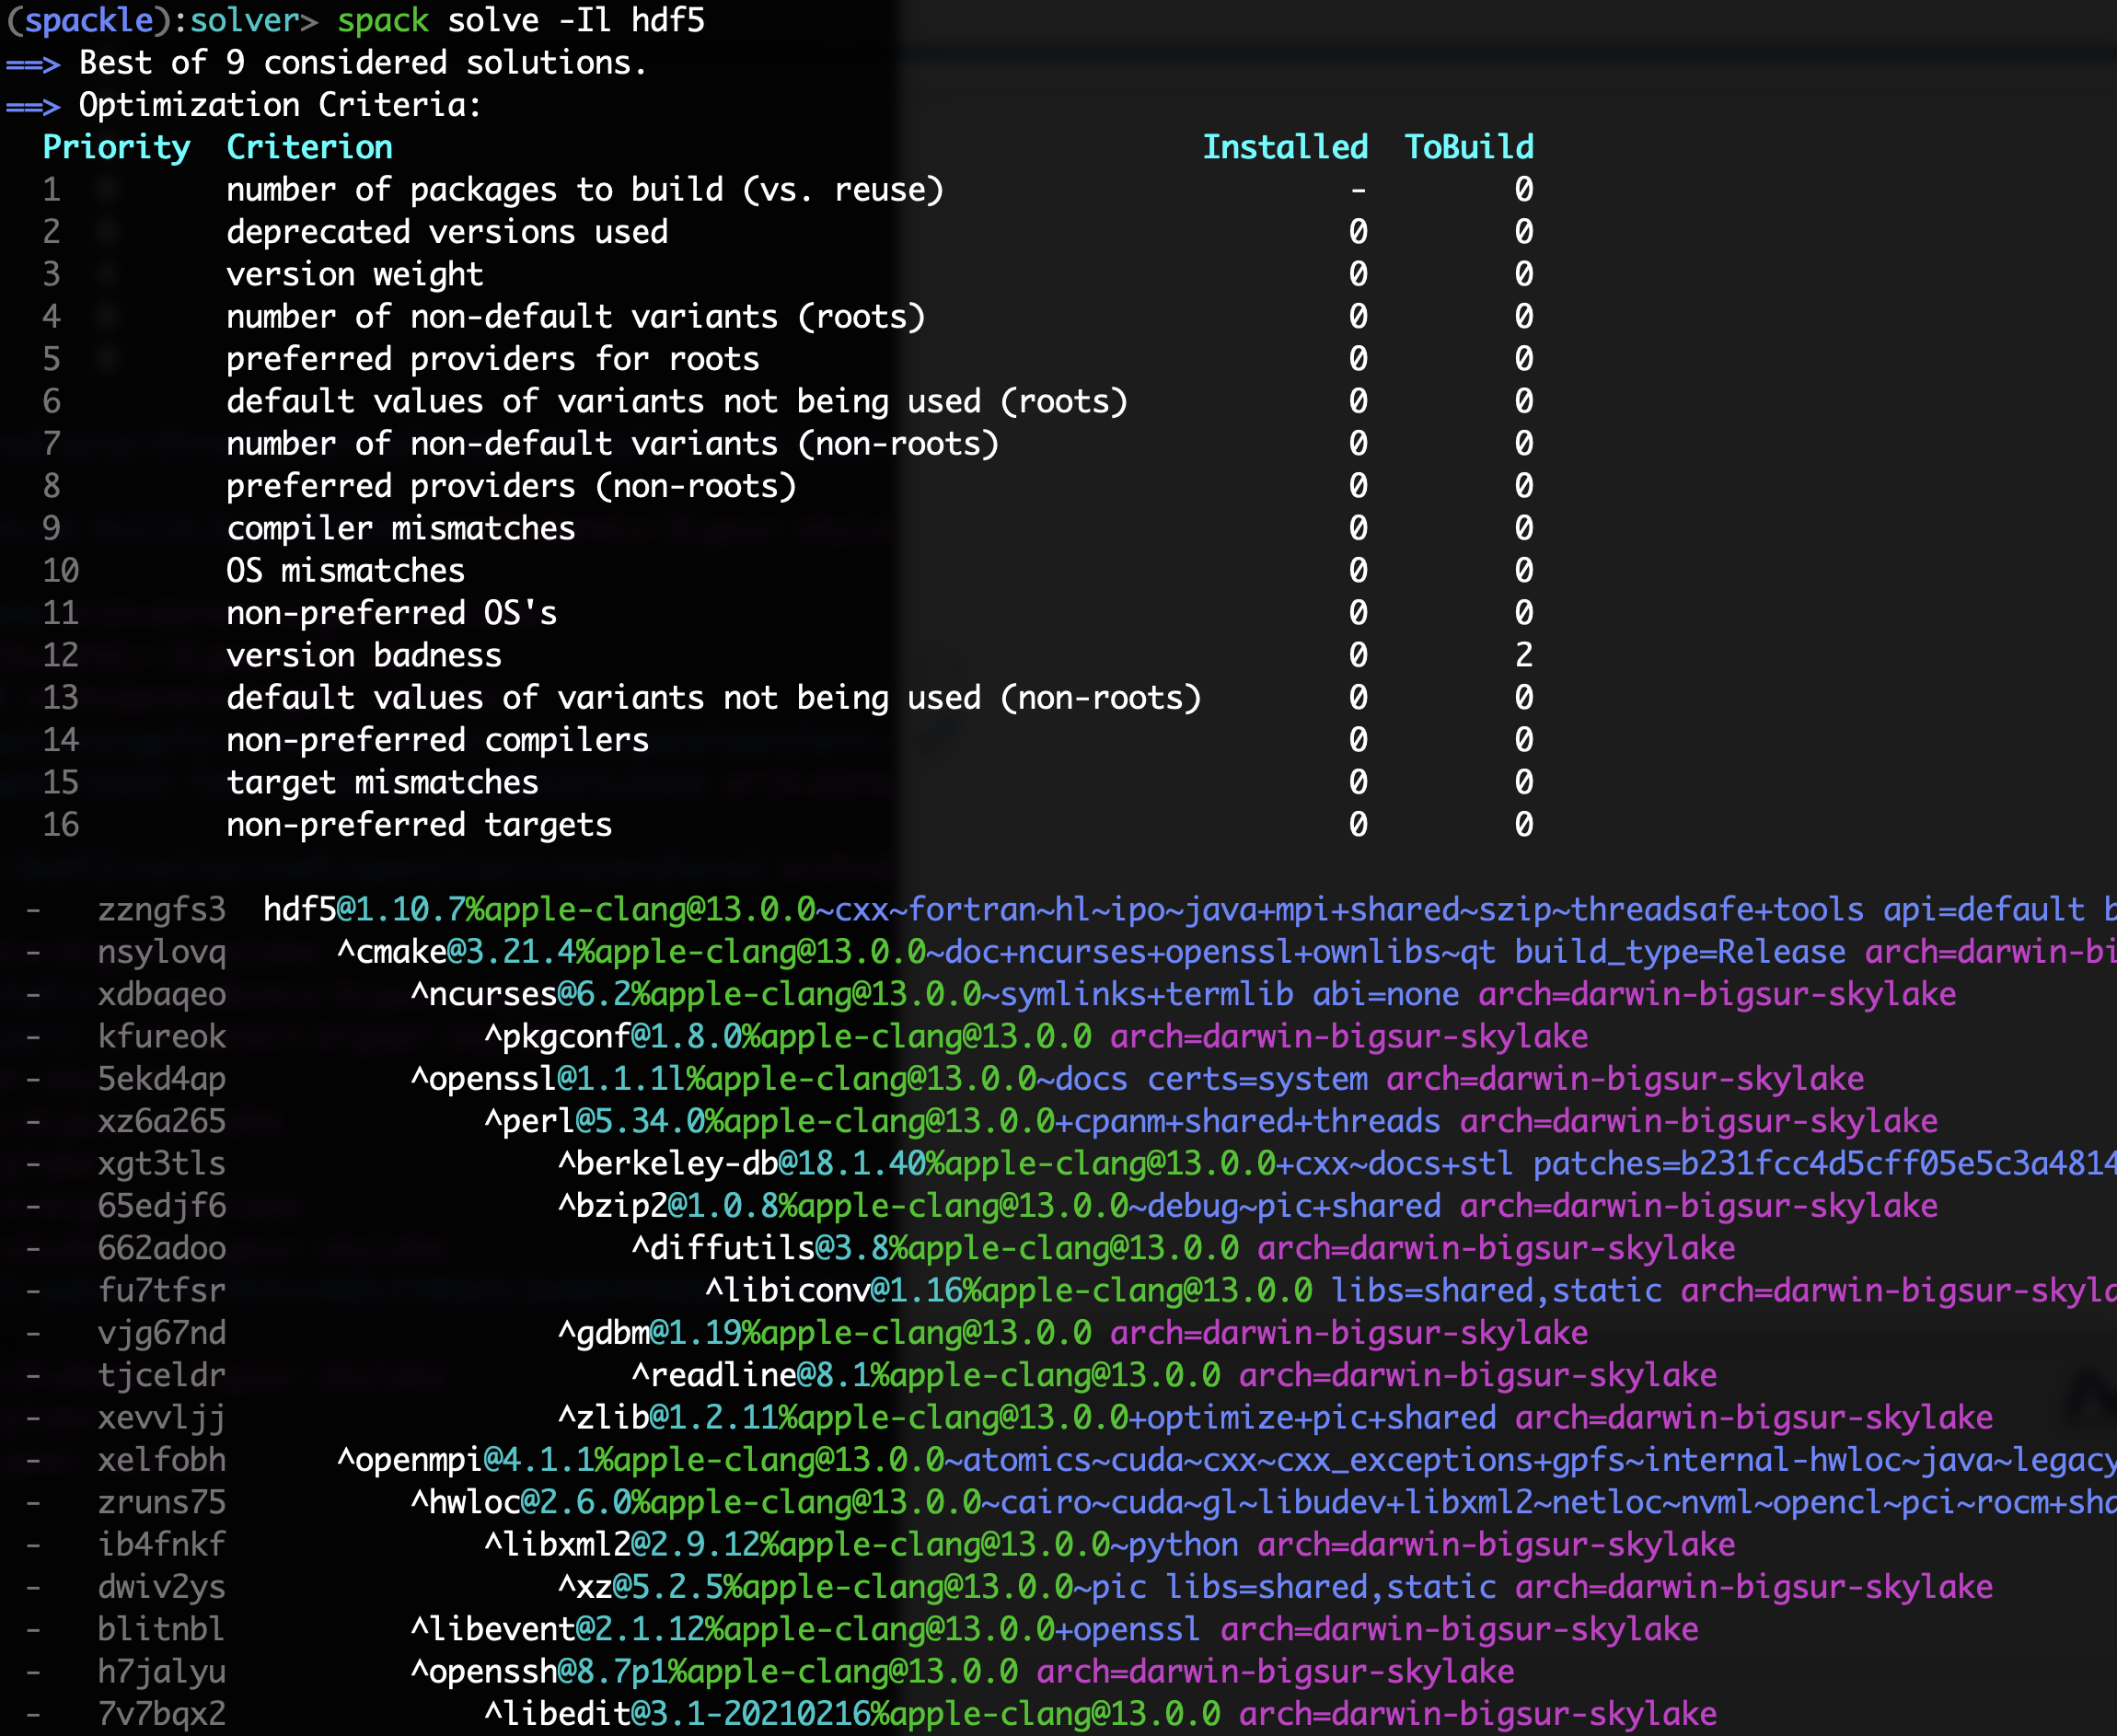
\includegraphics[width=2.4in]{figures/no-reuse.png}
    \label{fig:noreuse}
  }\\
%  \caption{Concretization of \texttt{hdf5} with pure hash-based reuse: all misses}
%\end{figure}
  %\begin{figure}[h]
  \subfloat[][Solving for reuse: 16 packages are actually acceptable]{
    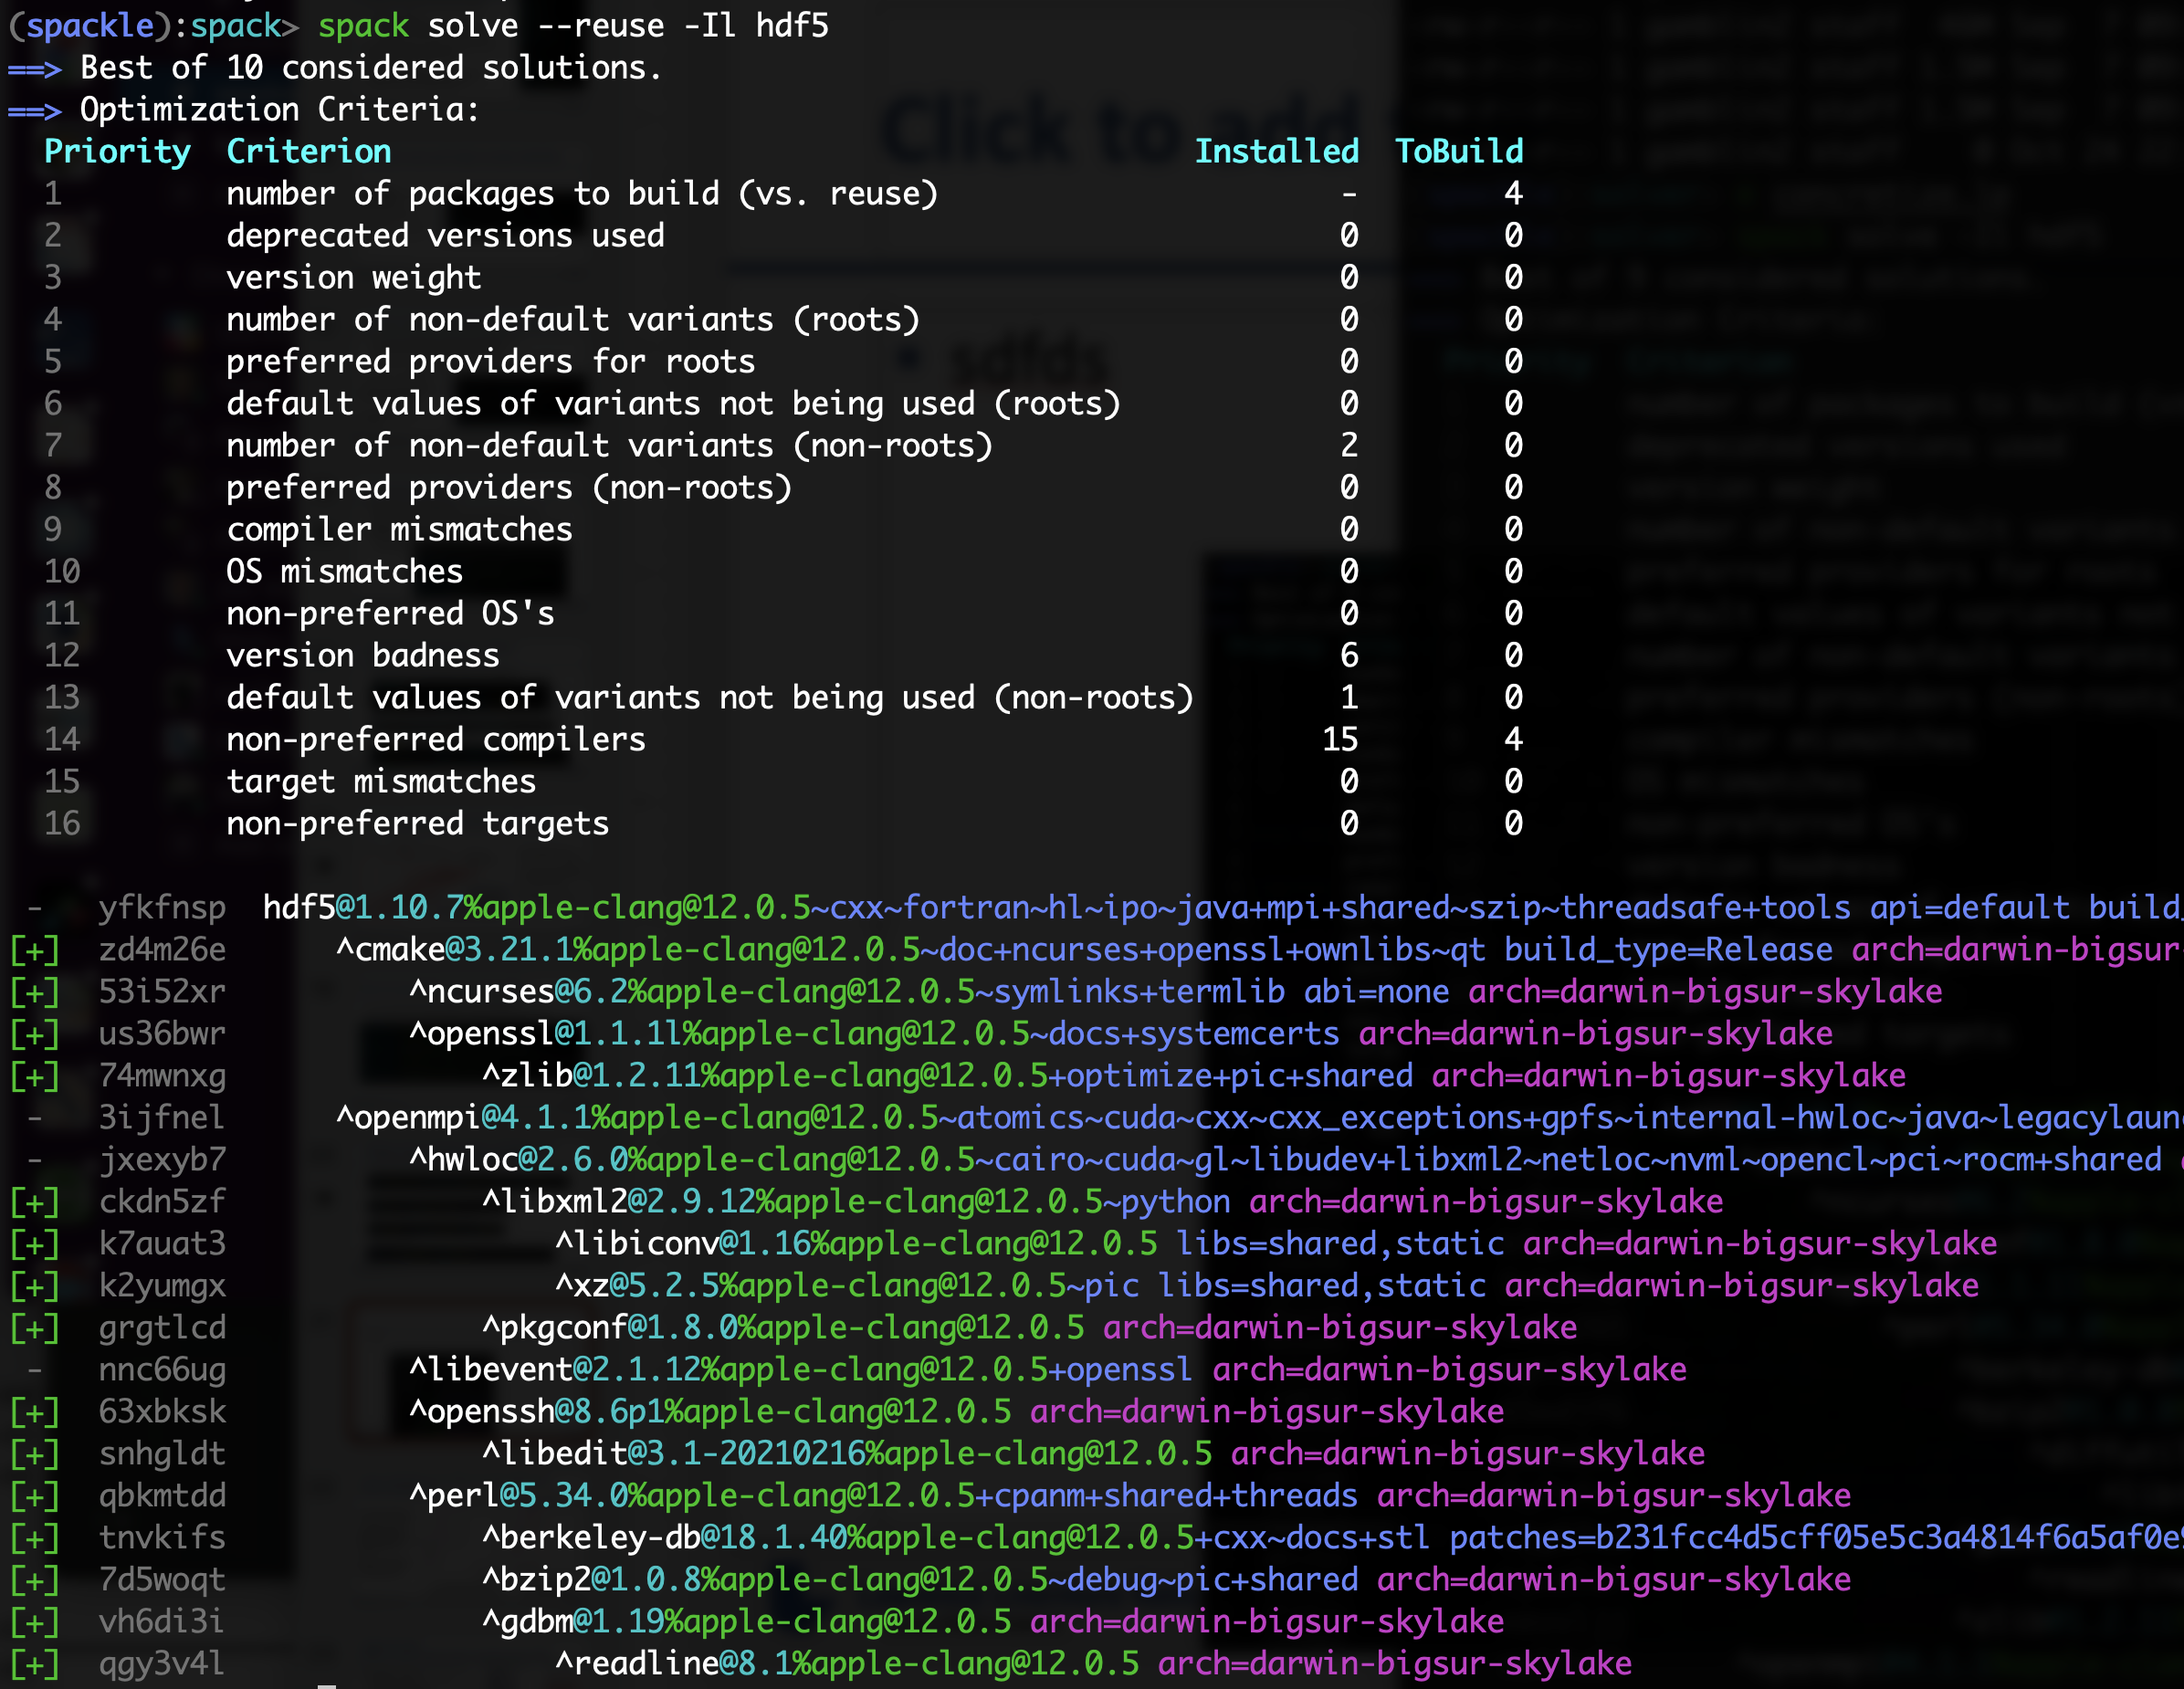
\includegraphics[width=2.4in]{figures/reuse.png}
    \label{fig:reuse}
  }
  \caption{Concretization with and without reuse optimization.}
  %\caption{The solver is asked to concretize \texttt{hdf5} trying to reuse installed software as much as possible. We see that 16 installed packages are actually acceptable to be reused. Another notable take is that, due to the priority chosen for minimizing the number of builds it is actually acceptable to \emph{reuse} \texttt{cmake} at version 3.21.1 even though the preferred version if it was to be built is 3.21.4}

\end{figure}


%- reuse of half the generalized condition
%- Reusing built dependencies
%- architecting optimization criteria for builds vs. reuse
